\documentclass{article}

\usepackage{tikz}
\usetikzlibrary{shapes.geometric, arrows, calc}

\tikzstyle{net} = [rectangle, text centered, draw=black, fill=blue!20]
\tikzstyle{cell} = [rectangle, minimum width=1.5cm, minimum height=1.5cm, text centered, draw=black, fill=green!20]
\tikzstyle{hidden_tensor} = [circle, minimum width=1cm, text centered, draw=black, fill=green!10]
\tikzstyle{output_tensor} = [circle, minimum width=1cm, text centered, draw=black, fill=orange!30]
\tikzstyle{input_tensor} = [circle, text centered, draw=black, fill=red!10]
\tikzstyle{add} = [circle, font=$+$, draw=black, text centered]
\tikzstyle{mul} = [circle, font=$\times$, draw=black, text centered]
\tikzstyle{arrow} = [thick,->,>=stealth]


\begin{document}

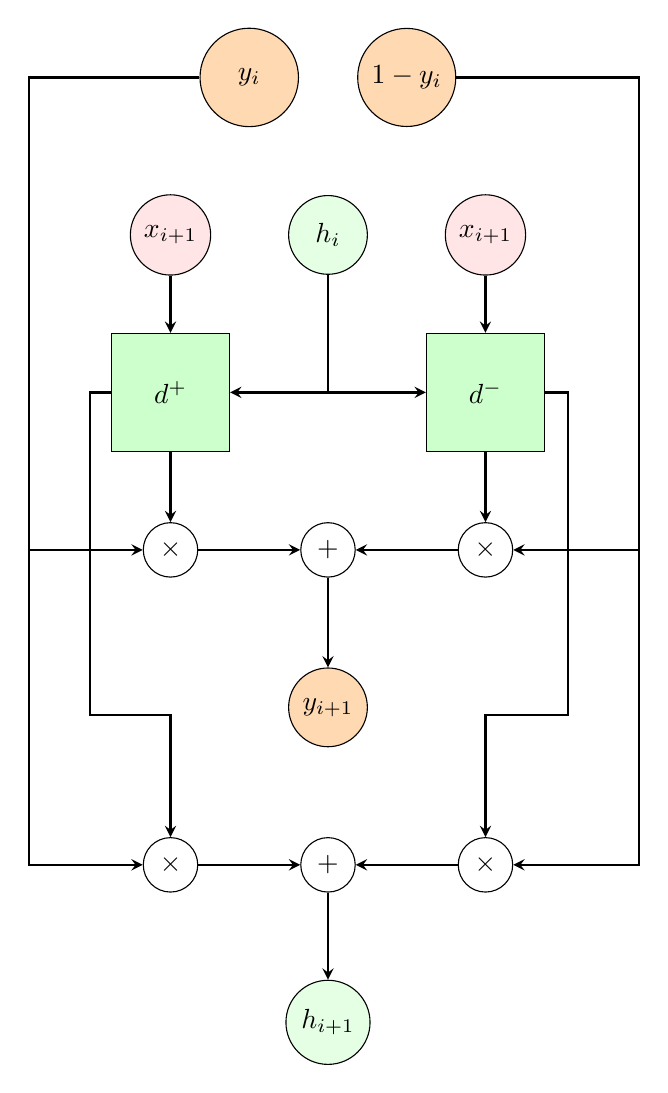
\begin{tikzpicture}[node distance=2cm]
    \node (yi)   [output_tensor, minimum width=1.25cm] {$y_i$};
    \node (one_m_yi)   [output_tensor, right of=yi] {$1-y_i$};
    
    \node (hi)   [hidden_tensor, below of=yi, xshift=1cm] {$h_i$};
    
    \node (dp)   [cell, left of=hi, yshift=-2cm] {$d^+$};
    \node (xip)   [input_tensor , above of=dp] {$x_{i+1}$};
    \node (mulpy) [mul, below of=dp] {};

    \node (dm)   [cell, right of=hi, yshift=-2cm] {$d^-$};
    \node (xim)   [input_tensor , above of=dm] {$x_{i+1}$};
    \node (mulmy) [mul, below of=dm] {};
    
    \node (addpmy) [add, right of=mulpy] {};
    \node (yi1) [output_tensor, below of=addpmy] {$y_{i+1}$};
    
    \node (addpmh) [add, below of=yi1] {};
    \node (mulph) [mul, left of=addpmh] {};
    \node (mulmh) [mul, right of=addpmh] {};

    \node (hi1) [hidden_tensor, below of=addpmh] {$h_{i+1}$};

%\draw [arrow] (yi) -- (one_m_yi);

\draw [arrow] (hi) |- (dp);
\draw [arrow] (xip) -- (dp);
\draw [arrow] (dp) -- (mulpy);
\draw [arrow] (yi) -| ($2.8*(xip)$)
                    |- (mulpy.west);
\draw [arrow] (mulpy) -- (addpmy);

\draw [arrow] (yi) -| ($2.8*(xip)$)
                    |- (mulph.west);


\draw [arrow] (dp) -| ($2.025*(dp)$)
                    -| (mulph.north);

\draw [arrow] (mulph) -- (addpmh);

\draw [arrow] (hi) |- (dm);
\draw [arrow] (xim) -- (dm);
\draw [arrow] (dm) -- (mulmy);
\draw [arrow] (one_m_yi.east) -| ($1.65*(xim)$)
                               |- (mulmy);
\draw [arrow] (mulmy) -- (addpmy);

\draw [arrow] (dm) -| ($1.35*(mulmy)$)
                    -| (mulmh.north);

\draw [arrow] (one_m_yi.east) -| ($1.65*(xim)$)
                               |- (mulmh);
\draw [arrow] (mulmh) -- (addpmh);

\draw [arrow] (addpmy) -- (yi1);
\draw [arrow] (addpmh) -- (hi1);


\end{tikzpicture}


\end{document}